\begin{figure}[!ht]
\begin{subfigure}{\linewidth}
\centering
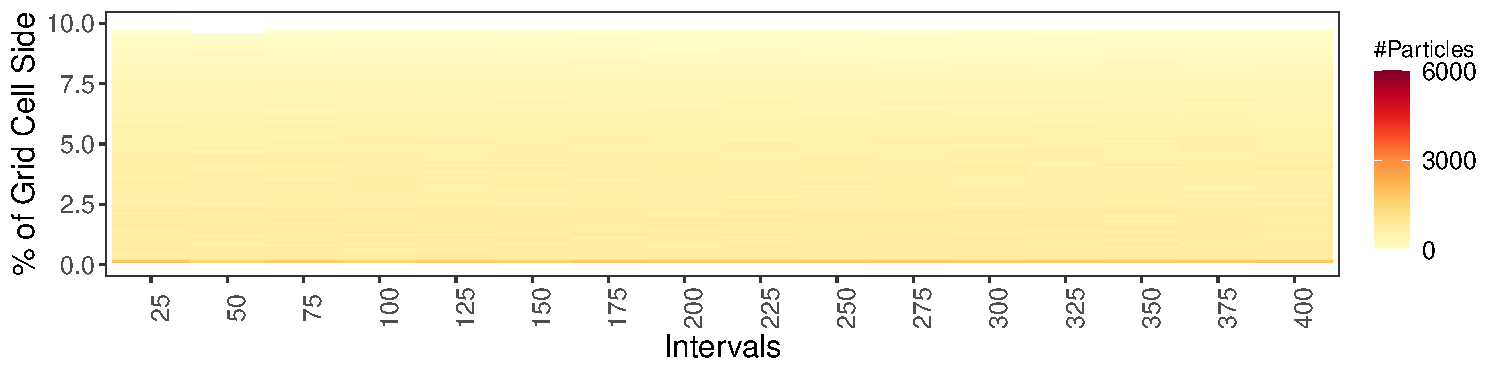
\includegraphics[width=0.95\linewidth]{Images/ABC_Intervals_T4.pdf}
\caption{T4, storage interval = 25 cycles}
\label{fig:abc_4}
\end{subfigure}
\begin{subfigure}{\linewidth}
\centering
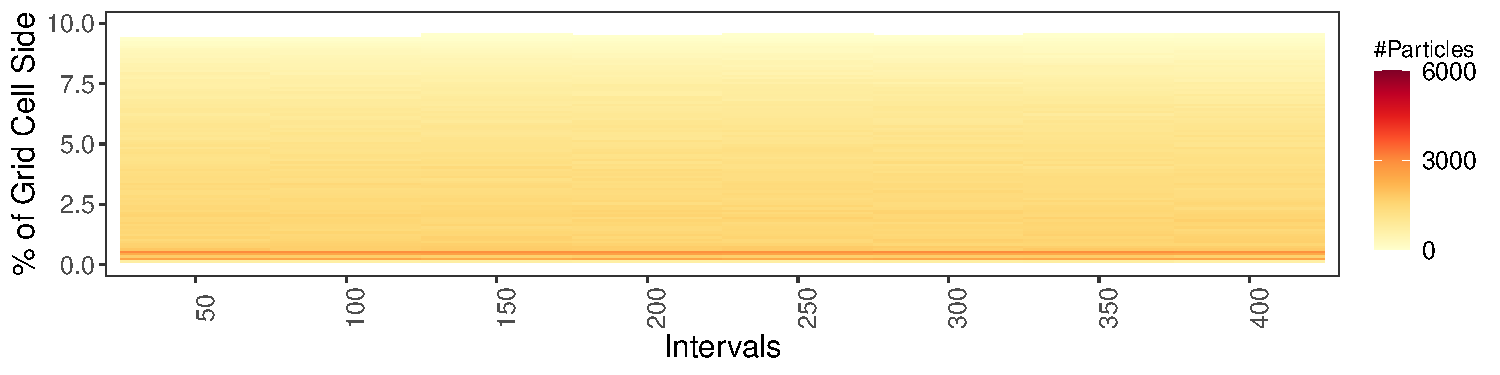
\includegraphics[width=0.95\linewidth]{Images/ABC_Intervals_T5.pdf}
\caption{T5, storage interval = 50 cycles}
\label{fig:abc_5}
\end{subfigure}
\begin{subfigure}{\linewidth}
\centering
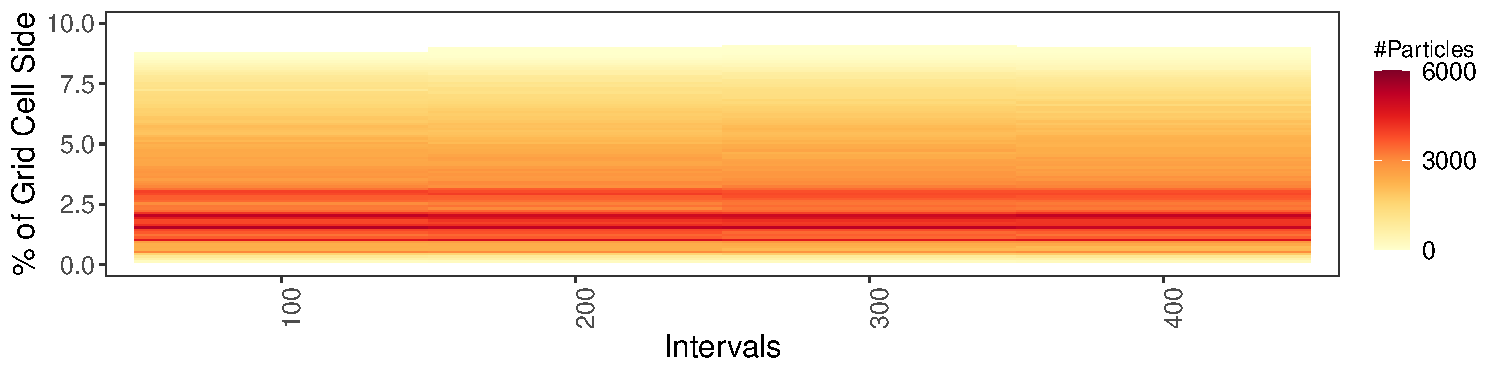
\includegraphics[width=0.95\linewidth]{Images/ABC_Intervals_T6.pdf}
\caption{T6, storage interval = 100 cycles}
\label{fig:abc_6}
\end{subfigure}
%\caption{Reconstruction error of varying storage intervals for the ABC data set.}
\caption{ABC data set tests showing impact of variation in storage interval on the distribution of reconstruction error.}
\label{fig:abc_map}
\end{figure}
